\lecture{LECTURE: Local Area Networks (LANs)}{25-10-22}{09:00}{Amanda}{Zoom}

\section*{Network Interface Cards}
Any transmission from a Network Interface Card (NIC) will reach every other NIC. Each NIC has a unique LAN address, this is a 48-bit globally unique identifier called a Media Access Control (MAC) Address.

NICs read all broadcast messages and all multicast messages with addresses that they have been programmed to read. The hardware of the NIC will ignore all other addresses.
\subsection*{Media Access Control Addresses}
\marginNote{added 06-01-22}Media Access Control (MAC) addresses are written in hexadecimal and burnt into the read only memory (ROM). The manufacturer will assign a MAC address to a NIC. The MAC address is structured such that there is a manufacturer identifier part and a unique device identifier part. 

\section*{Ethernet LAN Access Devices}
Client devices can have a cable between their PC and an interconnection device in a network rack. These interconnection devices could be: a hub; a switch; or a router.

\section*{Access and Distribution Rules}
\subsection*{Shared Media LANs}
Shared media LANs can only support a limited number of users and will generally be limited by their size. It shares its total bandwidth between all the devices connected.
\begin{figure}[H]
    \begin{minipage}[t]{0.45\textwidth}
        \textbf{Access Rules for Ethernet Hubs}
        \begin{itemize}
            \item Listen before sending
            \item Stop if multiple users start at the same time
        \end{itemize}
    \end{minipage}\hfill
    \begin{minipage}[t]{0.45\textwidth}
        \textbf{Distribution Rules for Ethernet Hubs}
        \begin{itemize}
            \item All traffic goes everywhere (NICs on receiving devices will pick out which packets are for it)
            \item One packet at a time
        \end{itemize}
    \end{minipage}\hfill
\end{figure}
There can still be collisions.
\begin{figure}[H]
    \centering
    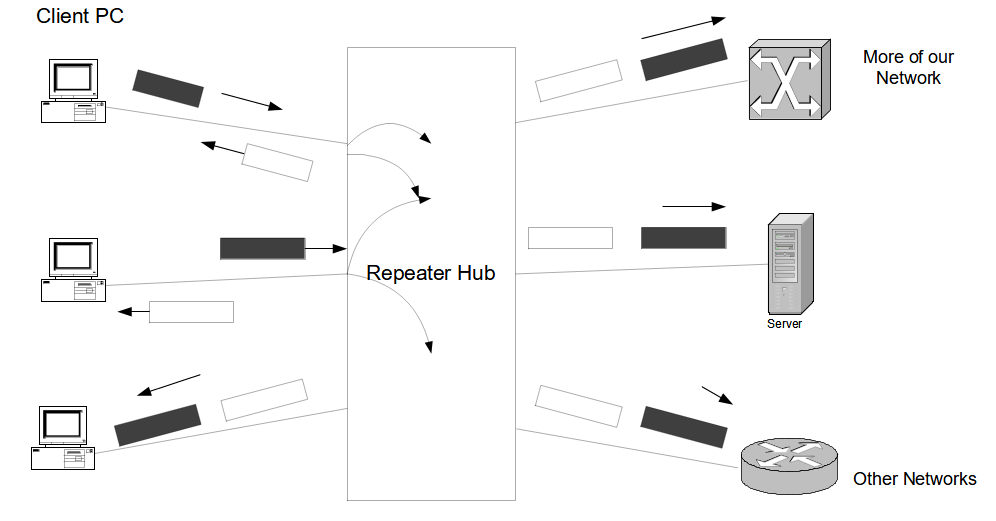
\includegraphics[width=0.8\textwidth]{assets/access-distro-shared-media-lans.png}
    \caption{Diagram of packet transmission on a shared media LAN}
\end{figure}
\subsection*{Switched Ethernet LANs}
\begin{figure}[H]
    \begin{minipage}[t]{0.45\textwidth}
        \textbf{Access Rules for switched Ethernet}
        \begin{itemize}
            \item Send whenever you want
            \item No collisions
        \end{itemize}
    \end{minipage}\hfill
    \begin{minipage}[t]{0.45\textwidth}
        \textbf{Distribution Rules for switched Ethernet}
        \begin{itemize}
            \item Traffic only goes where it needs to go
            \item Multiple Ethernet frames can be flowing
        \end{itemize}
    \end{minipage}\hfill
\end{figure}
This LAN works by the packet arriving at the switch, it looking at the header of the packet and determining which route the packet should take to reach its destination. The switch sends the packet to the correct destination only. If the packet needs to go to multiple destinations, multicast has to be used. 
\begin{figure}[H]
    \centering
    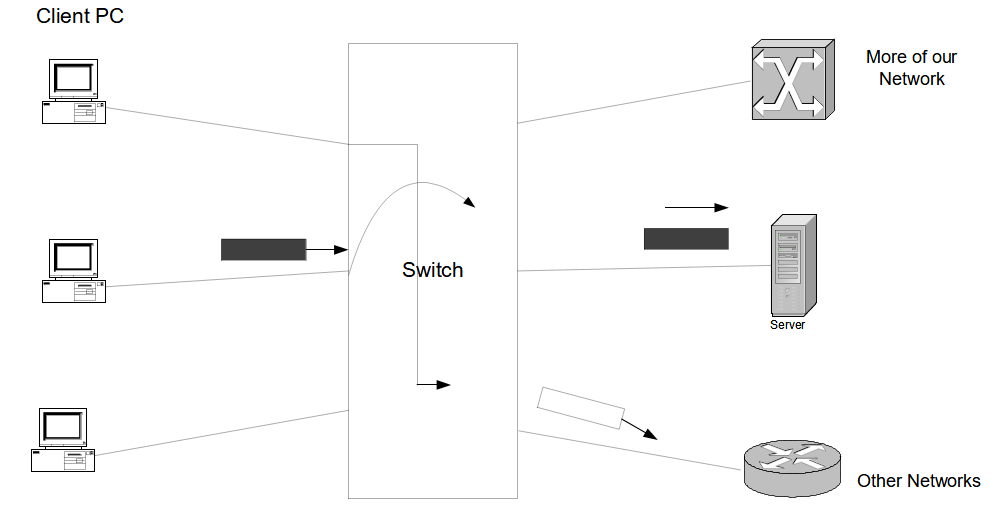
\includegraphics[width=0.8\textwidth]{assets/access-distro-switched-ethernet.png}
    \caption{Diagram of packet transmission on a switched Ethernet LAN}
\end{figure}
Switched Ethernet is a hardware implementation of bridging. Switched Ethernet automatically learns  address; forwards selectively to the destination; supports many ports per switch; supports full duplex on dedicated ports. 

Switches can support different data rates on each port. Ethernet switches will generally operate in \textit{store and forward} mode, this is where they temporarily hold the frame whilst making the forwarding decisions. Some Ethernet switches may also support \textit{cut-through operation}, which is where they start to forward after receiving the destination address part of the frame; this can only happen if the output port id is free and of the same data rate. Cut-through reduces the delay of the packet getting through the switch.

\section*{Classification of Transmission}
Unicast - single destination addressing. This specifies a single node on the network to transmit to.

Multicast - multiple but not all destinations addressing. This transmits packets to all nodes in a target group. Not all destinations. The same packet is duplicated by the switch to go our on multiple ports.

Broadcast - all destinations. This transmits packets to all nodes on a network. Hubs will broadcast to all devices connected. Switches can broadcast to all devices connected if the address says it can. 

\section*{The LAN Networking Model}
LANs operate at the \textit{data link} layer of the Reference Model. IEEE has divided the data link layer into two sub-layers: Logical Link Control (LLC); and Media Access Control (MAC).

Quality Of Service lives in the MAC sub-layer.
\subsection*{IEEE 802}
As seen in the diagram below, there are a number of different LAN standards. They all come under the IEEE 802 standards.
\begin{figure}[H]
    \centering
    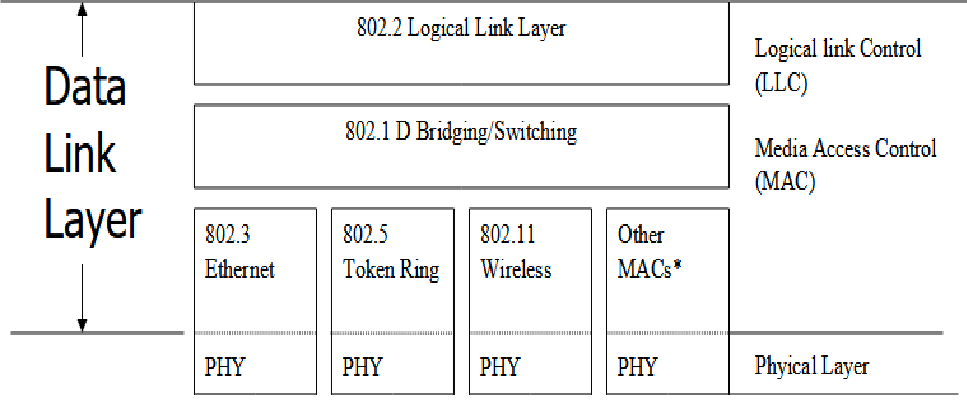
\includegraphics[width=0.8\textwidth]{assets/802-layers.png}
    \caption{Diagram of the 802 LAN Standards}
\end{figure}
802 is often pronounced "eighty-two". 
\subsection*{Common Aspects of the LAN standards}
All standards use the same MAC address length (48 bits); support broadcast and multicast addressing; and all have good (32-bit) error checking.
\subsection*{Different Aspects of the LAN standards}
There are a number of differences between some of the LAN standards: access methods (some use CSMA/CD while some use token passing); maximum frame size; support for features (for example priority) is only available in some standards; and specific data rate values.
\subsection*{Virtual LANs}
Virtual LANs (VLANs) are pieces of software which give an appearance of a physical connection. Their purpose is to limit broadcast traffic to a defined group (workgroup). The workgroup is defined by network management. Membership is setup by selecting a set of ports on a switch; selecting a set of MAC addresses; or Layer 3 protocol type (for example IP or IPX). The network administrator configures the VLAN membership, this is much better than re-cabling. Multiple VLANs can be configured and one VLAN can connect to another VLAN.
\subsection*{Power over Ethernet}
Power over Ethernet (PoE) utilizes the Ethernet cabling to deliver power to some Ethernet attached devices, for example: ethernet telephones; or wireless access points. PoE is defined in standard 802.3af.

The advantages of PoE are that power outlets may not be near and backup power may not be available in everyone's offices.

\section*{Ethernet Standards}
\begin{table}[H]
    \centering
    \begin{tabularx}{0.9\textwidth}{X|X}
        Standard & Properties\\
        \hline
        10 BASE5 (thickWire Ethernet) & 10mbit/s, baseband, 500m maximum\\
        10 BASE2 (thinWire Ethernet) & 10mbit/s, baseband, 185m maximum\\
        10 BASE-T & 10mbit/s, baseband, 100m maximum. Uses unsheilded twisted pair (UTP)\\
        10 BASE-F & Fibre optic Ethernet (10mbit/s)\\
        10 BASE-T and 100 BASE-F & 10mbit/s, baseband\\        
    \end{tabularx}
    \caption{Variations of IEEE 802.3}
\end{table}

There are a number of 1Gigabit/s Ethernet standards aswell: 10GBASE-T UTP (Gigabit Ethernet, GbE); 10GBASE-x Fibre; 40GBBASE-X Fibre; and 100GBASE-X Fibre.

\subsection*{10 BASE-T}
This is a multiport repeater. It can support up to four hubs (four repeater sets) along a data path. It can carry 10 mbit/s over two-pair Category 3 or better cabling. It supports up to 100m of cable length from the hub.

\subsection*{100 BASE-T}
This is a direct extension of 10 BASE-T. It can carry 100Mbit/s over two-pair category 5e UTP (fast Ethernet). It can support up to 100m of cable length from the hub and two 100BASE-T switches can be interconnected.

\subsection*{Gigabit Ethernet}
There are a number of different gigabit Ethernet standards.
\begin{table}[H]
    \centering
    \begin{tabularx}{0.9\textwidth}{X|XXXX}
    \textbf{IEEE} & \textbf{Designation} & \textbf{Data Rate} & \textbf{Media Type} & \textbf{Max segment length} \\
    \hline
    \multirow{3}{*}{802.3z} & 1000BASE-SX 850nm & 1000 mbit/s & 50 micron MMF & 500m \\
     & 1000BASE-SX 850nm & 1000 mbit/s & 62.5 micron MMF & 275m \\
     & 1000BASE-LX 1300nm & 1000 mbit/s & Single Mode Fibre & 5000m \\
    802.3ab & 1000BASE-T & 1000 mbit/s & Cat 5e UTP & 100m \\
    802.3an & 10GBASE-T & 10000 mbit/s & UTP & 100m \\
    802.3ae & 10GBASE-X & 10Gbps & SMF or MMF & 40km \\
    802.3ba & 40GBASE-X & 40Gbps & MMF or SMF & 40km \\
    802.3ba & 100GBASE-X & 100Gbps & MMF or SMF & 40km\\
    \end{tabularx}
\end{table}
\subsection*{802/3ae}
There is a never ending demand for higher-data-rate communications. Despite the higher-data-rate capabilities, some things never change: 802.3/ Ethernet frame format; same minimum and maximum frame sizes; and same structured cabling topologies all stay the same. However, there are some things which do change (for 1 and 10Gbit/s), there is no CSMA/CD and it only uses full duplex communication. 10Gbit/s will be used in MANs, large networks and SANs; it is a replacement for SONET/ SDH networks.

\subsection*{Legacy Ethernet}
\begin{table}[H]
    \centering
    \begin{tabularx}{0.6\textwidth}{X|XX}
     & \textbf{ThickWire} & \textbf{ThinWire} \\
    \hline
    Current Status & Legacy & Legacy \\
    Specification & 802.3 & 802.3 \\
    Data Rates & 10 Mbit/s & 10 Mbit/s \\
    Topology & Bus & Bus \\
    Cabling & Special coax & RG-58 coax \\
    Connectors & Attachment Unit Interface & BayoNet connector \\
    Max. Cable Length & 500m & 185m \\
    Max repeaters & 4 & 4\\
    \end{tabularx}
\end{table}

\subsection*{Contemporary Ethernet}
\begin{table}[H]
    \centering
    \begin{tabularx}{0.8\textwidth}{X|XXXX}
     & \textbf{Ethernet} & \textbf{Fast Ethernet} & \textbf{Gigabit Ethernet} & \textbf{10G Ethernet} \\
    \hline
    Current Status & Mature & Mature & Current & Current \\
    Specification & 802.3 & 802.3u & 802.3z, 802.3ab & 802.3ae \\
    Data Rate & 10 Mbit/s & 100 Mbit/s & 1000 Mbit/s & 10 Gbit/s \\
    Topology & Star/ Tree & Star & Star & Stat \\
    Cabling & Cat 3 to 5e UTP & Cat 3 to 5e UTP & Fibre & Fubre \\
    Connectors & RJ-54 & RJ-45 & SC, MT-RJ or RJ-45 & Fibre Optic Connectors \\
    Max. Cable Length & 100m & 100m & Varies & Varies \\
    Max. hubs & 4 & 2 & N/A & N/A
    \end{tabularx}
\end{table}

\section*{Ethernet Frame Format}
The diagram below shows the Ethernet Frame Format.
\begin{figure}[H]
    \centering
    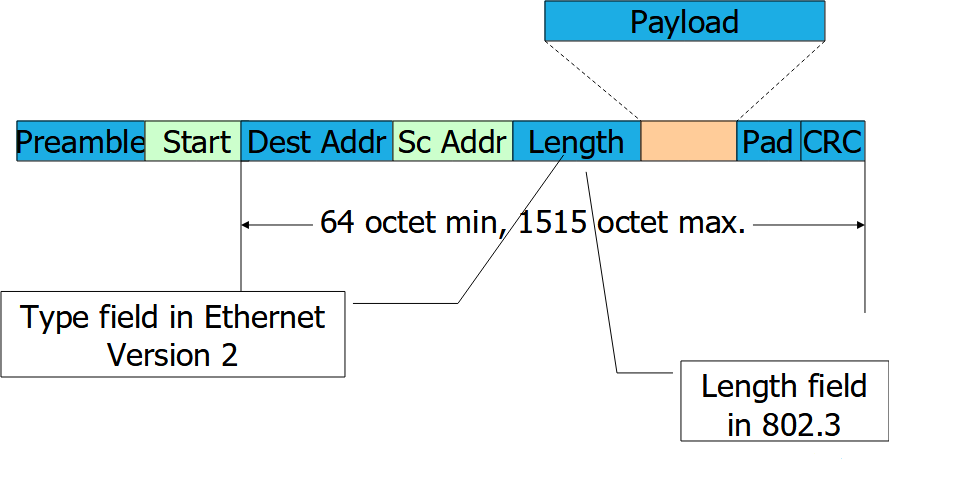
\includegraphics[width=0.8\textwidth]{assets/ethernet-frame-format.png}
    \caption{Ethernet Frame Format according to IEEE 802.3}
\end{figure}